% Springer LNNS (Lecture Notes in Networks and Systems) paper generated from the outputs of mlforle12.py
% Compile: pdflatex main && pdflatex main   (or: tectonic main.tex)
% Uses Springer's proceedings class llncs.cls, the template LNNS uses (on CTAN / TeX Live / Overleaf).
% The appendix table and figures are produced by make_paper_assets.py.
\documentclass[runningheads]{llncs}

\usepackage[T1]{fontenc}
\usepackage[utf8]{inputenc}
\usepackage{graphicx}
\usepackage{booktabs}
\usepackage{longtable}
\usepackage{pdflscape}
\usepackage{amsmath}
\usepackage{cite}
\usepackage{tikz}
\usetikzlibrary{positioning,arrows.meta}
\usepackage{xurl}
\usepackage[hidelinks]{hyperref}
\graphicspath{{life_figures/}}

\begin{document}

\title{An Experimental Framework for Life Expectancy Prediction from Single-Country Life-Factor Data}
\titlerunning{Life Expectancy Prediction from Single-Country Data}

% Author block kept commented for anonymous review; uncomment for the camera-ready version.
% \author{Asina Bopushova\inst{1} \and Ruslan Isaev\inst{2}}
% \authorrunning{A. Bopushova and R. Isaev}
% \institute{Computer Science Department, Ala-Too International University, Bishkek, Kyrgyzstan \and
% Computing Department, Westminster International University in Tashkent, Tashkent, Uzbekistan}

\maketitle

\begin{abstract}
Life-expectancy prediction from person-level risk factors is usually studied on a small cohort
from one country, which limits data volume and transferability. We propose an experimental
framework that combines any person-wise life-factor dataset with public life tables to predict
life expectancy for the reference country and for every country with a life table. A Kyrgyz
cohort of 95 participants, collected with a cyber-physical system, is labelled with the remaining
life expectancy $e(x)$ of the 2023 Kyrgyz life table. It is modelled with a mean baseline, a direct
life-table lookup, Ridge, Random Forest (RF) and Gradient Boosting (GB), and re-labelled with the
tables of 192 countries. A built-in audit separates circular target construction from validation
design. Because the labels are a function of age, the lookup reproduces them exactly, and the
cross-validated R$^2$ of 0.96 of the learned models comes from age (97--98\% of SHAP). Without age
and its proxies, RF and GB do not beat the mean baseline, a limitation of the labelling scheme
rather than evidence against lifestyle effects. A separate life-table forecaster, evaluated at five
rolling origins (2019--2023), found naive persistence hardest to beat (pooled MAE 0.79 years), and
feature ablations trace the learned models' failures to momentum features.
\keywords{Life expectancy \and Data leakage \and SHAP \and Life tables \and Transferability \and Kyrgyzstan}
\end{abstract}

%---------------------------------------------------------------------------
\section{Introduction}

Life expectancy is studied at two levels. At the \emph{population} level, demographic and
Bayesian models project it for every country~\cite{raftery2013,foreman2018,schumacher2025}, and
machine-learning (ML) models on country indicators now report R$^2$ above
0.98~\cite{chinthaginjala2026a,chinthaginjala2026b,ahamad2025}. At the \emph{individual} level,
lifestyle risk factors such as smoking, diet, physical activity and body mass index can separate
survival by decades within one country~\cite{jackowska2024}. Wearables and smart scales now make
such person-level data cheaper to collect~\cite{bopushova2026}.

The two levels rarely meet. Individual-level models assume one domestic mortality baseline, while
cross-country studies find that structural and country-level factors, not personal habits,
explain most of the variation in life
expectancy~\cite{chinthaginjala2026b,vladimirskaya2023,visbal2026}. A model built on one country's
cohort therefore faces three problems: person-level data are \emph{scarce}, results do not
\emph{generalise} automatically to other mortality regimes, and they are hard to \emph{reproduce}
and audit. Age is a legitimate predictor of remaining life expectancy, but when the target
\emph{is} the life-table value for the participant's age, a model that sees age recovers the table,
and its accuracy reflects this circularity~\cite{kaufman2012} rather than a learned effect of
lifestyle.

We generalise a Kyrgyz study in which a cyber-physical system with a smart scale and lifestyle
monitoring collected risk factors~\cite{bopushova2026} into a proposed experimental framework that
links person-level data to population life tables. Its contributions are:
(i)~a pipeline that anchors any person-wise life-factor dataset to a reference life table and
re-labels it under any country's mortality schedule;
(ii)~an audit that separates circular target construction from validation design;
(iii)~rolling-origin forecasting of life tables for 192 countries against simple
baselines~\cite{hyndman2021}, with feature ablations;
(iv)~per-country status and feature importance (Appendix~\ref{app:countries}).

%---------------------------------------------------------------------------
\section{Related Work}

\textbf{Population-level forecasting.} Classical methods extrapolate age-specific mortality, most
prominently Lee--Carter~\cite{leecarter1992}. The UN adopted Bayesian hierarchical projections of
life expectancy for all countries~\cite{raftery2013}. The Global Burden of Disease study forecasts
and estimates mortality for 195--204 countries~\cite{foreman2018,schumacher2025}. Multi-population
models show that stable relationships often hold only within clusters of similar
countries~\cite{levantesi2023}, and trajectories diverge through shocks such as
COVID-19~\cite{aburto2022}. For short horizons, the naive forecast remains the standard
benchmark~\cite{hyndman2021}.

\textbf{ML on country indicators.} Tree ensembles~\cite{breiman2001,friedman2001} and stacking
models trained on country panels reach high accuracy with drivers such as income, health
expenditure, undernourishment and governance~\cite{chinthaginjala2026a,ahamad2025,zhang2025,visbal2026}.
The determinants differ by development level: communicable disease and basic living conditions
matter most in low-income countries, and non-communicable disease and behaviour in high-income
ones~\cite{vladimirskaya2023,zhang2025}. Attribution analyses find that country-level structure
dominates, which argues for country-held-out validation before claims of
generalisation~\cite{chinthaginjala2026b}.

\textbf{Individual level and validation.} Life-table models extended with lifestyle factors
quantify personal risk within one country~\cite{jackowska2024}, and sensor-based systems collect
such factors continuously~\cite{bopushova2026}. Leakage inflates reported performance when target
information enters the features or the validation split~\cite{kaufman2012}. Grouped
cross-validation is recommended for clustered data~\cite{roberts2017}, and permutation
tests~\cite{ojala2010} and SHAP~\cite{lundberg2017,lundberg2020} check whether and how a model uses
its inputs. Our framework bridges these lines and builds such checks into the pipeline.

%---------------------------------------------------------------------------
\section{Proposed Experimental Framework}

\begin{figure}[t]
\centering
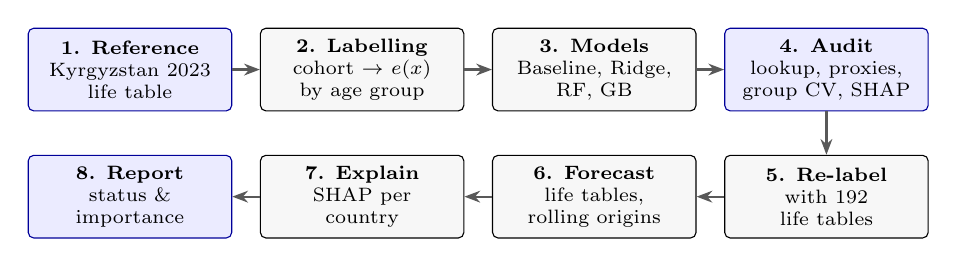
\begin{tikzpicture}[
  box/.style={draw, rounded corners=2pt, align=center, font=\scriptsize, minimum height=1.05cm, text width=2.35cm, fill=gray!6},
  hl/.style={box, fill=blue!8, draw=blue!60!black},
  arr/.style={-{Stealth[length=2mm]}, thick, gray!70!black}]
\node[hl]  (ref)  {\textbf{1. Reference}\\Kyrgyzstan 2023\\life table};
\node[box, right=0.35cm of ref]  (lab)  {\textbf{2. Labelling}\\cohort $\to$ $e(x)$\\by age group};
\node[box, right=0.35cm of lab]  (mod)  {\textbf{3. Models}\\Baseline, Ridge,\\RF, GB};
\node[hl, right=0.35cm of mod]   (aud)  {\textbf{4. Audit}\\lookup, proxies,\\group CV, SHAP};
\node[box, below=0.55cm of aud]  (tra)  {\textbf{5. Re-label}\\with 192\\life tables};
\node[box, left=0.35cm of tra]   (fc)   {\textbf{6. Forecast}\\life tables,\\rolling origins};
\node[box, left=0.35cm of fc]    (exp)  {\textbf{7. Explain}\\SHAP per\\country};
\node[hl, left=0.35cm of exp]    (rep)  {\textbf{8. Report}\\status \&\\importance};
\draw[arr] (ref) -- (lab); \draw[arr] (lab) -- (mod); \draw[arr] (mod) -- (aud);
\draw[arr] (aud) -- (tra); \draw[arr] (tra) -- (fc); \draw[arr] (fc) -- (exp); \draw[arr] (exp) -- (rep);
\end{tikzpicture}
\caption{Proposed experimental framework. Person-wise life-factor data from one country are
labelled with that country's life table, modelled and audited, then re-labelled and forecast for
every country with a life table.}
\label{fig:framework}
\end{figure}

Figure~\ref{fig:framework} shows the framework. Its inputs are \emph{any} person-wise life-factor
table with age and risk factors, and a set of abridged life tables; nothing is specific to
Kyrgyzstan or to the chosen features. Its two components share only the life tables. The
\emph{cohort component} (steps 1--5) labels and models person-level data. The \emph{life-table
component} (step 6) forecasts the tables from their own history and uses no cohort data. It
supplies tables for years not yet published, which step 2 can use to label a cohort for a future
year. All steps use scikit-learn~\cite{pedregosa2011} with fixed seeds.

\textbf{Design goals.} The framework \emph{addresses}, but does not remove, three problems.
(1)~\emph{Data scarcity}: life tables label the cohort for 192 countries without new data, but a
small cohort limits which effects can be learned (Sect.~\ref{sec:leak}).
(2)~\emph{Generalisability}: re-labelling the same participants only rescales their labels; showing
that person-level relations hold elsewhere requires cohorts from other countries.
(3)~\emph{Reproducibility}: public life tables, fixed seeds and one script regenerate all results,
given access to the cohort data.

\textbf{Data.} The cohort~\cite{bopushova2026} has 95 participants and 30 variables. They are aged
16--65 (median 19; 63 aged 15--19), 24\% are female, and mean BMI is $22.2\pm4.0$. We use the
study's 12 features: age, sex, BMI, sleep, steps per day, physical activity, smoking, alcohol, body
water, muscle mass, body fat and chronic disease. Cleaning fixes the decimal format and trailing
spaces that created spurious categories, encodes physical activity ordinally and imputes one
missing muscle-mass value with the median. The abridged life tables come from the United Nations
World Population Prospects 2024~\cite{wpp2024}. They cover 192 countries for 2015--2023 with 19 age
groups, giving $q_x$, $l_x$ and $e_x$ (no missing values), and are used as published;
preprocessing only parses age groups and builds lagged panels. Code: \url{https://github.com/Data-Analysis-and-Research-Institute/life-expectancy-kg-to-192}.
Ethics: non-invasive, anonymised data from volunteers; no formal approval was sought
[\textbf{TODO: exemption rule; consent, incl.\ parental for ages 16--17}].

\textbf{Labelling and models.} For country $c$ and year $t$, participant $i$ of age $a_i$
receives $y_i^{(c)} = e^{(c,t)}_{x(a_i)}$ with $x(a)=\max\{x_k : x_k\le a\}$. The reference is
Kyrgyzstan in 2023, which replaces the fixed table of~\cite{bopushova2026}; that table lies about
2.8 years above the 2023 values at young ages. Two reference predictors bracket the learned
models: a mean baseline, and a direct \emph{life-table lookup} $\hat y_i=e_{x(a_i)}$, which
reproduces the labels exactly. Between them we train Ridge, RF (200 trees) and GB (200 stages,
learning rate 0.05; library defaults otherwise), evaluated on an 80/20 split, as
in~\cite{bopushova2026}, and with $5\times5$ repeated $k$-fold CV (mean of the 25 fold MAEs).
Augmentation appends two copies of the 76 training rows with Gaussian noise (SD 1\% of each
feature's training SD) on the seven continuous features (age, BMI, sleep, steps, body water, muscle
mass, body fat); labels are unchanged and the 19 test rows stay clean.

\textbf{Target and validation audit.} We separate two issues. (i)~\emph{Circular target
construction}: $y$ is a step function of age, so a model with access to age or its proxies can
recover the lookup. This is not train--test contamination. Augmentation is train-only, and no
fitted statistic crosses folds except the median imputation of one value. (ii)~\emph{Validation
design}: random folds place participants of the same age group, who share one label, in both
training and test sets, so models interpolate between known labels. Leave-one-age-group-out CV
instead tests prediction at unseen ages. Regularised RF and GB (depth $\le4$, $\ge5$ samples per
leaf) are run in five scenarios: (A)~all features, random 5-fold CV; (B)~all features, age-group
CV; (C)~no age; (D)~no age and no age proxies; (E)~D with age-group CV. Proxies have
$|\rho_\text{Spearman}|\ge0.2$ with age, a threshold in the largest gap of the correlation profile
(BMI 0.35, body fat 0.24, all others $\le0.14$); we also test 0.1, 0.3 and 0.4. One 5-fold split
and pooled out-of-fold predictions are used throughout. Gains over the mean baseline get 95\%
intervals from a paired bootstrap over participants (2000 resamples). Permutation tests refit each
model on 100 permuted targets with the same folds, with
$p=(1+\#\{\text{MAE}_\text{perm}\le\text{MAE}_\text{obs}\})/101$ (minimum 0.01). Random-CV
scenarios shuffle labels across participants; age-group-CV scenarios permute which label each
group carries, because a global shuffle would break the constant-label groups and give an easier
null.

\textbf{Re-labelling and forecasting.} The cohort is re-labelled with each country's 2023 table,
a counterfactual that asks what this cohort's labels would be under another mortality schedule. For
life-table forecasting, $e_x$ in year $t$ is predicted from $e_{t-1..t-3}$, their changes
$\Delta$, $\log q_{x,t-1}$, the country's $e^0_{t-1}$ and its change, and the age group. Learned
models predict $e_t-e_{t-1}$. We compare naive persistence, a per-series linear trend, and global
Ridge, RF and histogram GB at every feasible origin (2019--2023; 2018 is the first year with three
lags), each trained only on earlier years. A \emph{selected} forecaster picks the model with the
lowest mean error at earlier origins, and ablations remove one feature group at a time. Four series
with a single-year $e^0$ change above 10 years (Central African Republic, Holy See, South Sudan,
State of Palestine; next largest 6.4) are excluded and reported separately.

%---------------------------------------------------------------------------
\section{Results}

\textbf{Starting point.} Kyrgyz $e^0$ fell 1.7 years in 2020 and reached 71.8 in 2023, rank 116
of 192 and 1.9 years below the world median; Kazakhstan, Russia, Uzbekistan and Tajikistan are
ahead and Turkmenistan behind.

\subsection{Cohort Models}

Table~\ref{tab:models} reproduces the ranking of~\cite{bopushova2026}: GB, then RF, then Ridge,
all far better than the mean baseline. The direct lookup, however, is exact (MAE 0, R$^2$ 1), so the
learned models only approximate a function known in closed form. Our errors exceed those reported,
consistent with the corrected life table and the clean test set. With \emph{age alone}, GB reaches
a CV MAE of 0.20 years; without age, the MAE rises to 4.4--4.8 years.

\begin{table}[t]
\centering
\caption{Cohort models, Kyrgyzstan 2023 target (years): 80/20 hold-out, augmented hold-out,
$5\times5$ repeated CV, and MAE reported in~\cite{bopushova2026}.}\label{tab:models}
\scriptsize
\begin{tabular}{@{}lrrrrrrr@{}}
\toprule
Model & MAE & RMSE & R$^2$ & MAE (aug.) & CV MAE & CV R$^2$ & MAE~\cite{bopushova2026} \\
\midrule
Life-table lookup & 0.00 & 0.00 & 1.00 & 0.00 & 0.00 $\pm$ 0.00 & 1.00 & -- \\
Baseline (mean) & 7.28 & 11.08 & 0.00 & 7.28 & 6.24 $\pm$ 1.35 & $-$0.11 & -- \\
Ridge & 1.24 & 1.59 & 0.98 & 1.19 & 1.21 $\pm$ 0.23 & 0.96 & 0.95 \\
Random Forest & 0.82 & 2.71 & 0.94 & 0.51 & 0.66 $\pm$ 0.54 & 0.95 & 0.39 \\
Gradient Boosting & \textbf{0.56} & 2.00 & 0.97 & \textbf{0.45} & \textbf{0.52} $\pm$ 0.53 & 0.96 & 0.18 \\
\bottomrule
\end{tabular}
\end{table}

\subsection{Target and Validation Audit}\label{sec:leak}

Table~\ref{tab:leak} uses regularised models and one pooled split, so its errors differ from
Table~\ref{tab:models}, which uses unregularised models and averages 25 fold MAEs (scenario A: RF
1.87, GB 0.99 vs.\ 0.66, 0.52). With age (A), RF and GB recover most of the lookup, and age takes
97--98\% of the mean $|$SHAP$|$. At unseen ages (B), GB still beats the group-permutation null
($p=0.01$) and RF does not ($p=0.17$). Without age (C), a gain remains, traced by SHAP to the proxy
BMI (3.2 years in RF, 6.1 in GB). Without proxies (D, E), neither model beats the baseline, and all
intervals include zero.

Pooled age-group errors are dominated by the 15--19 group (63 of 95; Table~\ref{tab:groups}); when
it is held out, only 32 older participants remain for training. Macro-averaged over groups, GB errs
by 4.6 years in B against 17.4 for the baseline, while in E all models lie within 0.1 years of it.
The result is robust to the threshold: removing only BMI (0.3) leaves gains of 1--7\% with
intervals spanning zero, 0.1 leaves both models at or below the baseline, and only keeping all
proxies (0.4) restores a gain (22--36\%). These negative results are a property of the labelling
scheme, not evidence against lifestyle effects: participants in an age group share one label, so
lifestyle can predict it only through its correlation with age.

\begin{table}[t]
\centering
\caption{Target and validation audit: pooled out-of-fold MAE (years), gain over the mean baseline
(95\% bootstrap interval) and permutation $p$.}\label{tab:leak}
\scriptsize\setlength{\tabcolsep}{4pt}
\begin{tabular}{@{}lrrrllr@{}}
\toprule
Scenario & Base & RF & GB & RF gain \% [CI] & GB gain \% [CI] & $p$ RF/GB \\
\midrule
A. All, random & 6.25 & 1.87 & 0.99 & 70 [63, 78] & 84 [79, 90] & -- \\
B. All, age-group & 12.31 & 6.48 & 4.70 & 47 [43, 52] & 62 [57, 66] & 0.17/0.01 \\
C. No age, random & 6.25 & 4.61 & 4.09 & 26 [13, 38] & 35 [19, 48] & 0.01/0.01 \\
D. No age/prox., random & 6.25 & 6.40 & 7.02 & $-$2 [$-$11, 5] & $-$12 [$-$29, 1] & 0.27/0.46 \\
E. No age/prox., age-group & 12.31 & 12.49 & 12.66 & $-$1 [$-$5, 2] & $-$3 [$-$12, 6] & 0.56/0.54 \\
\bottomrule
\end{tabular}
\end{table}

\begin{table}[t]
\centering
\caption{Leave-one-age-group-out CV: group size, label and MAE (years) per held-out age group for
scenarios B (all features) and E (no age, no proxies). The baseline is the same in B and E.}\label{tab:groups}
\scriptsize\setlength{\tabcolsep}{4pt}
\begin{tabular}{@{}lrrrrrrrrr|r@{}}
\toprule
Age group & 15--19 & 20--24 & 25--29 & 30--34 & 35--39 & 40--44 & 45--49 & 50--54 & 65--69 & Macro \\
\midrule
$n$ & 63 & 17 & 1 & 4 & 2 & 2 & 3 & 1 & 2 & \\
$e(x)$ & 58.16 & 53.30 & 48.48 & 43.66 & 38.91 & 34.34 & 29.96 & 25.72 & 14.21 & \\
\midrule
Baseline & 13.79 & 0.26 & 5.09 & 10.29 & 14.91 & 19.59 & 24.32 & 28.09 & 40.15 & 17.39 \\
RF (B) & 6.85 & 4.10 & 3.84 & 4.90 & 3.26 & 3.03 & 6.66 & 10.05 & 24.37 & 7.45 \\
GB (B) & 4.69 & 4.43 & 0.78 & 4.05 & 3.89 & 1.29 & 3.85 & 0.63 & 17.98 & 4.62 \\
RF (E) & 13.58 & 2.24 & 3.89 & 10.37 & 12.56 & 20.44 & 24.66 & 29.57 & 38.65 & 17.33 \\
GB (E) & 13.43 & 3.68 & 5.55 & 10.91 & 9.11 & 21.77 & 26.97 & 29.56 & 36.08 & 17.45 \\
\bottomrule
\end{tabular}
\end{table}

\subsection{Re-labelling with 192 Life Tables}

Under other countries' schedules, the cohort's mean label ranges from 43.5 to 68.8 years (Kyrgyzstan:
53.5). In all 192 label sets, age takes about 98\% of GB's SHAP importance and the model without age
and proxies never beats the baseline (Appendix~\ref{app:countries}). With participants fixed, this
shows the audit holds under any mortality schedule, \emph{not} that the models generalise to other
populations.

\subsection{Life-Table Forecasting}

On the 188 stable series (Table~\ref{tab:forecast}), learned models are marginally better only in
the calm year 2019; persistence or Ridge wins 2020--21, the trend the 2022 rebound, and persistence
2023. Pooled, persistence has the lowest MAE, RMSE and 95th-percentile error and is best in 107
countries, including Kyrgyzstan (MAE 0.82). Selection on earlier origins switches between trend and
persistence and averages 1.09 over 2020--2023, against 0.94 for always using persistence.

\textbf{MAE versus RMSE.} On all 192 countries, persistence had the lowest 2023 MAE (0.69) but GB
the lowest RMSE (1.66 vs.\ 1.85). The gap comes from the four unstable series: persistence carries
the Central African Republic's 2022 value (18.9 years) into 2023 (published 57.4), a 38-year error
that dominates RMSE. Without them, persistence also has the lowest 2023 RMSE (0.80 vs.\ 1.04), so
no trade-off remains; on them, no model is reliable (MAE 2--7 years at every origin). The Central
African Republic's published $e^0$ for 2015--2023 reads 51.9, 51.0, 45.1, 52.2, 31.5, 50.6, 40.1,
18.9, 57.4, passed unchanged by our preprocessing. The earlier RF projection of 35.3 years for 2024
was the momentum features' reversal of the +38.5-year jump, so we report no projections for
unstable series.

\textbf{Ablations.} SHAP ranks a recent change ($\Delta_{t-2}$) first in 107 countries; ablations
show that this reliance hurts. Removing the momentum features lowers GB's mean MAE from 0.92 to
0.89, and a level-only model (age group, $e_{t-1}$) to 0.84 (RF: 0.93 to 0.87), mostly in 2021--23.
Removing the country's $e^0$ raises it (0.96); deeper lags and $\log q$ have no effect. The models
fail by extrapolating recent changes across regime shifts, and even the level-only model does not
beat persistence (0.84 vs.\ 0.79).

\begin{table}[t]
\centering
\caption{Rolling-origin forecasting of $e_x$, 188 stable series $\times$ 19 ages (years). Wins:
countries with the lowest mean MAE. Selected: best model at earlier origins.}\label{tab:forecast}
\scriptsize\setlength{\tabcolsep}{4pt}
\begin{tabular}{@{}lrrrrrrrrr@{}}
\toprule
 & \multicolumn{5}{c}{MAE by forecast year} & \multicolumn{3}{c}{Pooled 2019--23} & \\
\cmidrule(lr){2-6}\cmidrule(lr){7-9}
Model & 2019 & 2020 & 2021 & 2022 & 2023 & MAE & RMSE & P95 & Wins \\
\midrule
Naive (persistence) & 0.19 & \textbf{0.85} & 0.88 & 1.46 & \textbf{0.56} & \textbf{0.79} & \textbf{1.21} & \textbf{2.68} & 107 \\
Linear trend & \textbf{0.17} & 0.95 & 1.11 & \textbf{1.09} & 1.06 & 0.88 & 1.27 & 2.70 & 29 \\
Ridge & 0.18 & 0.93 & \textbf{0.83} & 1.77 & 0.76 & 0.89 & 1.35 & 3.05 & 16 \\
Random Forest & \textbf{0.17} & 0.93 & 0.97 & 1.82 & 0.78 & 0.93 & 1.43 & 3.23 & 18 \\
Gradient Boosting & \textbf{0.17} & 0.93 & 0.94 & 1.77 & 0.79 & 0.92 & 1.40 & 3.21 & 18 \\
Selected (earlier years) & -- & 0.95 & 0.88 & 1.46 & 1.06 & & & & \\
\bottomrule
\end{tabular}
\end{table}

%---------------------------------------------------------------------------
\section{Discussion and Conclusion}

The framework produces reproducible life-table labels for one cohort under 192 mortality
schedules. Its audit shows that a life-table target measures how well a model reads the table: the
lookup is exact, and the accuracy of such designs, including~\cite{bopushova2026}, comes from age.
The weak lifestyle-only models reflect this labelling scheme, not an absence of the lifestyle effects
reported elsewhere~\cite{chinthaginjala2026b,vladimirskaya2023,jackowska2024}. Feature effects need a
target that varies between individuals, such as survival or health outcomes collected by the
cyber-physical system, and population claims need cohorts from other countries. For the life
tables, persistence was the strongest forecaster across origins, so the latest published table is
the best basis for next-year labels, and ML forecasters must be reported against it.
\emph{Limitations}: a small, young, urban cohort; tables not split by sex; only five forecast
origins, four in or after COVID-19.

%---------------------------------------------------------------------------
\begin{thebibliography}{99}

\bibitem{aburto2022}
Aburto, J.M., Schöley, J., Kashnitsky, I., et al.: Quantifying impacts of the COVID-19 pandemic
through life-expectancy losses: a population-level study of 29 countries. International Journal of
Epidemiology \textbf{51}(1), 63--74 (2022)

\bibitem{ahamad2025}
Ahamad, S.S., Kumar, K.P., Ganesh, S.S., et al.: Machine learning-based life expectancy prediction
in developed and developing regions. IEEE Access \textbf{13}, 69520--69531 (2025).
\doi{10.1109/ACCESS.2025.3560890}

\bibitem{bopushova2026}
Bopushova, A., Isaev, R.: Design and implementation of cyber-physical data collection system of
risk factors mitigation and life expectancy prediction. In: 2026 International Conference on
Computer Systems and Technologies (CompSysTech), pp.~1--6. IEEE, Ruse, Bulgaria (2026).
\doi{10.1109/CompSysTech69798.2026.11683147}

\bibitem{breiman2001}
Breiman, L.: Random forests. Machine Learning \textbf{45}(1), 5--32 (2001)

\bibitem{chinthaginjala2026a}
Chinthaginjala, R., Tera, S.P., Natha, P., et al.: A multi-stage stacking framework for accurate
and interpretable life expectancy modeling. PLOS One \textbf{21} (2026).
\doi{10.1371/journal.pone.0353849}

\bibitem{chinthaginjala2026b}
Chinthaginjala, R., Tera, S.P., El-Shafai, W., Azar, A.T., Kamal, N.A.: A scalable ensemble
learning framework for accurate and equitable global life expectancy prediction. In: 2026
International Conference on Control, Automation and Diagnosis (ICCAD), pp.~1--6. IEEE (2026).
\doi{10.1109/ICCAD69956.2026.11643040}

\bibitem{foreman2018}
Foreman, K.J., Marquez, N., Dolgert, A., et al.: Forecasting life expectancy, years of life lost,
and all-cause and cause-specific mortality for 250 causes of death: reference and alternative
scenarios for 2016--40 for 195 countries and territories. Lancet \textbf{392}, 2052--2090 (2018).
\doi{10.1016/S0140-6736(18)31694-5}

\bibitem{friedman2001}
Friedman, J.H.: Greedy function approximation: a gradient boosting machine. Annals of Statistics
\textbf{29}(5), 1189--1232 (2001)

\bibitem{hyndman2021}
Hyndman, R.J., Athanasopoulos, G.: Forecasting: Principles and Practice, 3rd edn. OTexts,
Melbourne (2021)

\bibitem{jackowska2024}
Jackowska, B., Wiśniewski, P., Noiński, T., Bandosz, P.: Effects of lifestyle-related risk factors
on life expectancy: a comprehensive model for use in early prevention of premature mortality from
noncommunicable diseases. PLOS One \textbf{19} (2024). \doi{10.1371/journal.pone.0298696}

\bibitem{kaufman2012}
Kaufman, S., Rosset, S., Perlich, C., Stitelman, O.: Leakage in data mining: formulation,
detection, and avoidance. ACM Transactions on Knowledge Discovery from Data \textbf{6}(4), 15 (2012)

\bibitem{leecarter1992}
Lee, R.D., Carter, L.R.: Modeling and forecasting U.S. mortality. Journal of the American
Statistical Association \textbf{87}(419), 659--671 (1992)

\bibitem{levantesi2023}
Levantesi, S., Nigri, A., Piscopo, G., Spelta, A.: Multi-country clustering-based forecasting of
healthy life expectancy. Quality \& Quantity, 1--27 (2023). \doi{10.1007/s11135-022-01611-6}

\bibitem{lundberg2017}
Lundberg, S.M., Lee, S.I.: A unified approach to interpreting model predictions. In: Advances in
Neural Information Processing Systems 30, pp. 4765--4774 (2017)

\bibitem{lundberg2020}
Lundberg, S.M., Erion, G., Chen, H., et al.: From local explanations to global understanding with
explainable AI for trees. Nature Machine Intelligence \textbf{2}, 56--67 (2020)

\bibitem{ojala2010}
Ojala, M., Garriga, G.C.: Permutation tests for studying classifier performance. Journal of
Machine Learning Research \textbf{11}, 1833--1863 (2010)

\bibitem{pedregosa2011}
Pedregosa, F., et al.: Scikit-learn: machine learning in Python. Journal of Machine Learning
Research \textbf{12}, 2825--2830 (2011)

\bibitem{raftery2013}
Raftery, A.E., Chunn, J.L., Gerland, P., Ševčíková, H.: Bayesian probabilistic projections of
life expectancy for all countries. Demography \textbf{50}, 777--801 (2013).
\doi{10.1007/s13524-012-0193-x}

\bibitem{roberts2017}
Roberts, D.R., et al.: Cross-validation strategies for data with temporal, spatial, hierarchical,
or phylogenetic structure. Ecography \textbf{40}(8), 913--929 (2017)

\bibitem{schumacher2025}
Schumacher, A.E., Zheng, P., Barber, R.M., et al.: Global age-sex-specific all-cause mortality and
life expectancy estimates for 204 countries and territories and 660 subnational locations,
1950--2023: a demographic analysis for the Global Burden of Disease Study 2023. Lancet
\textbf{406}, 1731--1810 (2025). \doi{10.1016/S0140-6736(25)01330-3}

\bibitem{visbal2026}
Visbal-Cadavid, D., Delahoz-Domínguez, E.J.: Modeling life expectancy through governance and
socioeconomic factors: a Bayesian network analysis. Journal of Sustainability Research (2026).
\doi{10.20900/jsr20260068}

\bibitem{vladimirskaya2023}
Vladimirskaya, A., Kolosnitsyna, M.: Factors in life expectancy: a cross-country analysis. Voprosy
Statistiki \textbf{30}(1), 70--89 (2023). \doi{10.34023/2313-6383-2023-30-1-70-89}

\bibitem{wpp2024}
United Nations, DESA, Population Division: World Population Prospects 2024. New York (2024).
\url{https://population.un.org/wpp/}

\bibitem{zhang2025}
Zhang, H., Qiao, H., Li, X., et al.: Determinants of life expectancy in high longevity countries:
evidence from machine learning. Frontiers in Public Health \textbf{13} (2025).
\doi{10.3389/fpubh.2025.1687871}

\end{thebibliography}

%---------------------------------------------------------------------------
\appendix
\begin{landscape}
\section{Prediction Status and Feature Importance for Every Country}\label{app:countries}

\small Kyrgyzstan comes first, then countries by $e^0_{2023}$. \emph{Status:} $\Delta$KGZ is the gap
to Kyrgyzstan; $\geq$2019 means $e^0_{2023}$ is at or above its 2019 level; Best/MAE give the
forecaster with the lowest mean MAE (years) over the 2019--2023 rolling origins; Naive is the
persistence MAE; Band is a \emph{retrospective error band} of that MAE (High $<0.5$, Med.\ $<1.5$,
Low), not an independently validated measure of forecastability; $^\dagger$ marks unstable source
series, which are not evaluated. \emph{Importance} (mean $|$SHAP$|$ of GB):
Age\% is age's share in the full cohort model; Non-age top is the strongest other feature; LF gain is
the CV MAE gain of the lifestyle-only model (no age, BMI, body fat) over the mean baseline, where
negative means no skill; LF top-2 are its largest features; Fcst.\ top is the top forecasting feature (share
\%). Full values are in \texttt{outputs/tables/}.

{\tiny\setlength{\tabcolsep}{4pt}\renewcommand{\arraystretch}{0.85}
\begin{longtable}{l r r r c l r r l r l r l l}
\caption{Prediction status and feature importance for all 192 countries (columns explained above).}\label{tab:app-countries}\\
\toprule
Country & $e^0_{23}$ & Rank & $\Delta$KGZ & $\geq$2019 & Best & MAE & Naive & Band & Age\% & Non-age top & LF gain & LF top-2 & Fcst. top (\%) \\
\midrule
\endfirsthead
\multicolumn{14}{l}{\emph{(continued)}}\\
\toprule
Country & $e^0_{23}$ & Rank & $\Delta$KGZ & $\geq$2019 & Best & MAE & Naive & Band & Age\% & Non-age top & LF gain & LF top-2 & Fcst. top (\%) \\
\midrule
\endhead
\bottomrule
\endfoot
\textbf{Kyrgyzstan} & 71.8 & 116 & +0.0 & yes & Naive & 0.82 & 0.82 & Med. & 98.5 & body fat & -12 & sleep, water & $\Delta$(t-1) (32) \\
Holy See$^\dagger$ & 88.7 & 1 & +17.0 & yes & -- & -- & -- & Unstable & 98.2 & body fat & -12 & water, sleep & $\Delta$(t-2) (75) \\
Rep. of Korea & 85.1 & 2 & +13.4 & yes & Trend & 0.65 & 0.80 & Med. & 98.4 & body fat & -13 & sleep, water & e0(t-1) (57) \\
Japan & 85.1 & 3 & +13.3 & yes & Ridge & 0.29 & 0.41 & High & 98.5 & activity & -13 & water, sleep & e0(t-1) (55) \\
Andorra & 84.8 & 4 & +13.0 & yes & Naive & 1.51 & 1.51 & Low & 98.5 & activity & -12 & sleep, water & $\Delta$(t-2) (35) \\
Singapore & 84.3 & 5 & +12.5 & yes & Naive & 0.28 & 0.28 & High & 98.5 & muscle & -13 & water, sleep & e0(t-1) (29) \\
Switzerland & 84.2 & 6 & +12.4 & yes & Trend & 0.44 & 0.58 & High & 98.4 & activity & -12 & sleep, water & $\Delta$(t-2) (53) \\
Australia & 84.1 & 7 & +12.3 & yes & Trend & 0.52 & 0.68 & Med. & 98.6 & body fat & -12 & water, sleep & e0(t-1) (35) \\
Malta & 84.0 & 8 & +12.3 & yes & Naive & 0.53 & 0.53 & Med. & 98.5 & activity & -13 & water, sleep & e0(t-1) (42) \\
Spain & 83.9 & 9 & +12.1 & yes & Trend & 0.63 & 0.83 & Med. & 98.5 & activity & -12 & water, sleep & $\Delta$(t-2) (59) \\
Italy & 83.9 & 10 & +12.1 & yes & Trend & 0.71 & 0.92 & Med. & 98.4 & body fat & -13 & water, sleep & $\Delta$(t-2) (43) \\
France & 83.5 & 11 & +11.8 & yes & Trend & 0.40 & 0.41 & High & 98.3 & activity & -12 & water, sleep & e0(t-1) (43) \\
Sweden & 83.4 & 12 & +11.7 & yes & Trend & 0.35 & 0.47 & High & 98.3 & activity & -12 & sleep, water & $\Delta$(t-2) (48) \\
UAE & 83.4 & 13 & +11.6 & yes & Ridge & 1.35 & 1.54 & Med. & 98.4 & body fat & -11 & water, sleep & $\Delta$(t-2) (68) \\
Norway & 83.2 & 14 & +11.5 & yes & Ridge & 0.24 & 0.33 & High & 98.4 & activity & -12 & water, sleep & e0(t-1) (42) \\
Canada & 82.9 & 15 & +11.1 & yes & Trend & 0.46 & 0.59 & High & 98.4 & body fat & -13 & water, sleep & e0(t-1) (31) \\
Qatar & 82.8 & 16 & +11.0 & no & Naive & 0.96 & 0.96 & Med. & 98.1 & body fat & -11 & water, sleep & $\Delta$(t-2) (38) \\
Iceland & 82.7 & 17 & +10.9 & no & RF & 0.33 & 0.61 & High & 98.6 & activity & -12 & water, sleep & $\Delta$e0(t-1) (43) \\
Ireland & 82.7 & 18 & +10.9 & no & Trend & 0.39 & 0.44 & High & 98.4 & activity & -13 & water, sleep & $\Delta$(t-2) (39) \\
Portugal & 82.6 & 19 & +10.8 & yes & Naive & 0.45 & 0.45 & High & 98.4 & activity & -12 & water, sleep & e0(t-1) (43) \\
Israel & 82.6 & 20 & +10.8 & no & Naive & 0.19 & 0.19 & High & 98.4 & body fat & -13 & water, sleep & $\Delta$(t-2) (36) \\
Luxembourg & 82.4 & 21 & +10.6 & yes & Naive & 0.32 & 0.32 & High & 98.4 & activity & -12 & sleep, water & $\Delta$e0(t-1) (41) \\
Belgium & 82.3 & 22 & +10.5 & yes & Trend & 0.59 & 0.81 & Med. & 98.6 & muscle & -13 & water, sleep & $\Delta$(t-2) (57) \\
Netherlands & 82.2 & 23 & +10.5 & yes & Naive & 0.36 & 0.36 & High & 98.4 & body fat & -13 & water, sleep & $\Delta$(t-2) (40) \\
New Zealand & 82.2 & 24 & +10.4 & yes & Ridge & 0.50 & 0.72 & Med. & 98.4 & activity & -13 & water, sleep & $\Delta$e0(t-1) (54) \\
Denmark & 82.0 & 25 & +10.3 & yes & Trend & 0.26 & 0.28 & High & 98.4 & activity & -12 & water, sleep & $\Delta$(t-1) (31) \\
Finland & 82.0 & 26 & +10.2 & no & Ridge & 0.26 & 0.34 & High & 98.5 & body fat & -13 & water, sleep & $\Delta$e0(t-1) (32) \\
Greece & 82.0 & 27 & +10.2 & yes & Ridge & 0.45 & 0.74 & High & 98.4 & muscle & -13 & water, sleep & $\Delta$(t-2) (51) \\
Austria & 81.9 & 28 & +10.1 & no & Trend & 0.34 & 0.43 & High & 98.4 & muscle & -13 & water, sleep & $\Delta$e0(t-1) (36) \\
Slovenia & 81.8 & 29 & +10.1 & yes & Naive & 0.51 & 0.51 & Med. & 98.5 & activity & -13 & water, sleep & $\Delta$(t-2) (40) \\
Cyprus & 81.7 & 30 & +10.0 & yes & Ridge & 0.31 & 0.47 & High & 98.4 & muscle & -13 & water, sleep & $\Delta$(t-2) (36) \\
Bahrain & 81.6 & 31 & +9.9 & yes & Naive & 1.16 & 1.16 & Med. & 98.4 & body fat & -12 & water, sleep & $\Delta$(t-2) (39) \\
Germany & 81.6 & 32 & +9.8 & yes & Trend & 0.37 & 0.54 & High & 98.4 & muscle & -12 & water, sleep & e0(t-1) (33) \\
Chile & 81.5 & 33 & +9.7 & yes & Naive & 0.85 & 0.85 & Med. & 98.5 & activity & -13 & water, sleep & $\Delta$(t-2) (40) \\
United Kingdom & 81.4 & 34 & +9.7 & no & Trend & 0.48 & 0.52 & High & 98.4 & muscle & -11 & water, sleep & $\Delta$(t-2) (37) \\
Costa Rica & 81.2 & 35 & +9.4 & yes & RF & 0.83 & 0.95 & Med. & 98.5 & muscle & -12 & water, sleep & $\Delta$(t-2) (51) \\
Maldives & 81.2 & 36 & +9.4 & yes & Naive & 0.93 & 0.93 & Med. & 98.4 & body fat & -11 & sleep, water & $\Delta$e0(t-1) (30) \\
Kuwait & 80.6 & 37 & +8.8 & yes & Ridge & 1.46 & 1.47 & Med. & 98.5 & water & -12 & water, sleep & $\Delta$(t-2) (58) \\
Panama & 80.1 & 38 & +8.3 & yes & Naive & 1.14 & 1.14 & Med. & 98.4 & body fat & -11 & water, sleep & e0(t-1) (31) \\
Oman & 80.0 & 39 & +8.3 & yes & Naive & 1.42 & 1.42 & Med. & 98.3 & body fat & -13 & sleep, water & $\Delta$(t-2) (39) \\
Anguilla & 79.9 & 40 & +8.2 & yes & Naive & 0.29 & 0.29 & High & 98.5 & water & -12 & water, sleep & e0(t-1) (22) \\
Czechia & 79.9 & 41 & +8.1 & yes & Naive & 0.89 & 0.89 & Med. & 98.4 & activity & -12 & water, sleep & $\Delta$(t-2) (34) \\
Albania & 79.7 & 42 & +8.0 & yes & Naive & 1.03 & 1.03 & Med. & 98.5 & water & -13 & water, sleep & $\Delta$(t-1) (36) \\
USA & 79.5 & 43 & +7.7 & yes & Naive & 0.91 & 0.91 & Med. & 98.5 & body fat & -12 & water, sleep & e0(t-1) (31) \\
Estonia & 79.3 & 44 & +7.5 & yes & Trend & 0.52 & 0.66 & Med. & 98.4 & activity & -12 & water, sleep & $\Delta$(t-2) (46) \\
Saudi Arabia & 79.0 & 45 & +7.2 & yes & GB & 0.58 & 0.65 & Med. & 98.4 & activity & -13 & water, sleep & $\Delta$(t-2) (34) \\
Poland & 78.8 & 46 & +7.0 & yes & Naive & 0.99 & 0.99 & Med. & 98.3 & body fat & -12 & sleep, water & $\Delta$(t-2) (33) \\
Croatia & 78.6 & 47 & +6.8 & yes & Naive & 0.47 & 0.47 & High & 98.4 & activity & -12 & water, sleep & $\Delta$(t-1) (39) \\
Slovakia & 78.5 & 48 & +6.7 & yes & GB & 1.26 & 1.39 & Med. & 98.5 & activity & -12 & sleep, water & $\Delta$(t-2) (60) \\
Uruguay & 78.3 & 49 & +6.5 & yes & GB & 0.84 & 1.22 & Med. & 98.4 & muscle & -12 & water, sleep & $\Delta$(t-2) (70) \\
Cuba & 78.2 & 50 & +6.5 & yes & Naive & 1.65 & 1.65 & Low & 98.5 & activity & -12 & sleep, water & $\Delta$(t-2) (67) \\
Peru & 78.2 & 51 & +6.5 & yes & GB & 1.90 & 2.10 & Low & 98.3 & body fat & -12 & water, sleep & $\Delta$(t-2) (62) \\
Jordan & 78.1 & 52 & +6.3 & yes & Naive & 1.22 & 1.22 & Med. & 98.5 & body fat & -12 & water, sleep & $\Delta$(t-2) (46) \\
China & 78.0 & 53 & +6.3 & no & Naive & 0.12 & 0.12 & High & 98.4 & activity & -12 & water, sleep & $\Delta$(t-2) (40) \\
Bosnia \& Herz. & 78.0 & 54 & +6.2 & yes & Naive & 1.35 & 1.35 & Med. & 98.4 & activity & -12 & water, sleep & $\Delta$(t-2) (51) \\
Lebanon & 77.9 & 55 & +6.1 & no & Naive & 1.50 & 1.50 & Low & 98.4 & body fat & -12 & water, sleep & $\Delta$(t-2) (59) \\
Antigua \& Barbuda & 77.8 & 56 & +6.1 & yes & Naive & 0.14 & 0.14 & High & 98.6 & body fat & -12 & water, sleep & $\Delta$e0(t-1) (37) \\
Colombia & 77.8 & 57 & +6.1 & yes & Naive & 1.48 & 1.48 & Med. & 98.5 & body fat & -12 & sleep, water & $\Delta$(t-2) (52) \\
Iran & 77.8 & 58 & +6.1 & yes & Naive & 1.26 & 1.26 & Med. & 98.3 & activity & -12 & sleep, water & e0(t-1) (41) \\
Sri Lanka & 77.6 & 59 & +5.8 & yes & Trend & 0.34 & 0.40 & High & 98.4 & activity & -12 & water, sleep & $\Delta$(t-2) (46) \\
Ecuador & 77.6 & 60 & +5.8 & no & Naive & 1.86 & 1.86 & Low & 98.3 & water & -13 & water, sleep & $\Delta$(t-1) (32) \\
Argentina & 77.5 & 61 & +5.7 & yes & Ridge & 1.02 & 1.07 & Med. & 98.5 & body fat & -12 & sleep, water & $\Delta$(t-2) (50) \\
North Macedonia & 77.5 & 62 & +5.7 & yes & Naive & 1.28 & 1.28 & Med. & 98.4 & activity & -12 & water, sleep & $\Delta$(t-2) (41) \\
Montenegro & 77.2 & 63 & +5.5 & yes & Ridge & 1.11 & 1.16 & Med. & 98.7 & body fat & -12 & sleep, water & $\Delta$(t-2) (58) \\
Türkiye & 77.2 & 64 & +5.5 & no & Naive & 0.87 & 0.87 & Med. & 98.5 & water & -12 & water, sleep & $\Delta$(t-1) (39) \\
Hungary & 77.1 & 65 & +5.3 & yes & Ridge & 0.93 & 0.94 & Med. & 98.5 & body fat & -12 & sleep, water & $\Delta$(t-2) (51) \\
Malaysia & 77.0 & 66 & +5.2 & yes & Ridge & 0.79 & 1.02 & Med. & 98.4 & body fat & -12 & water, sleep & $\Delta$(t-2) (52) \\
Serbia & 76.9 & 67 & +5.1 & yes & Naive & 1.30 & 1.30 & Med. & 98.5 & activity & -13 & sleep, water & $\Delta$(t-2) (46) \\
Thailand & 76.7 & 68 & +5.0 & no & Ridge & 0.43 & 0.55 & High & 98.2 & body fat & -12 & sleep, water & e0(t-1) (56) \\
Tunisia & 76.6 & 69 & +4.8 & yes & Naive & 1.16 & 1.16 & Med. & 98.5 & activity & -13 & water, sleep & $\Delta$(t-2) (56) \\
Aruba & 76.6 & 70 & +4.8 & yes & Naive & 0.88 & 0.88 & Med. & 98.6 & muscle & -13 & water, sleep & $\Delta$(t-2) (54) \\
Algeria & 76.4 & 71 & +4.6 & yes & Naive & 1.00 & 1.00 & Med. & 98.3 & activity & -13 & water, sleep & $\Delta$(t-2) (40) \\
Latvia & 76.3 & 72 & +4.5 & yes & RF & 0.92 & 1.06 & Med. & 98.5 & body fat & -12 & sleep, water & $\Delta$(t-2) (58) \\
Cabo Verde & 76.2 & 73 & +4.4 & yes & Naive & 0.73 & 0.73 & Med. & 98.4 & body fat & -12 & water, sleep & $\Delta$e0(t-1) (55) \\
Barbados & 76.1 & 74 & +4.4 & no & Ridge & 0.18 & 0.32 & High & 98.5 & activity & -12 & water, sleep & e0(t-1) (46) \\
Lithuania & 76.1 & 75 & +4.3 & no & Ridge & 0.73 & 0.78 & Med. & 98.6 & BMI & -12 & sleep, water & e0(t-1) (47) \\
Romania & 76.0 & 76 & +4.2 & yes & Naive & 1.04 & 1.04 & Med. & 98.6 & body fat & -13 & water, sleep & $\Delta$(t-2) (37) \\
Brazil & 75.9 & 77 & +4.2 & no & Naive & 0.94 & 0.94 & Med. & 98.4 & body fat & -11 & water, sleep & $\Delta$(t-2) (34) \\
Armenia & 75.8 & 78 & +4.1 & yes & Naive & 1.59 & 1.59 & Low & 98.6 & body fat & -12 & sleep, water & e0(t-1) (52) \\
Bulgaria & 75.6 & 79 & +3.9 & yes & Ridge & 1.28 & 1.35 & Med. & 98.6 & body fat & -13 & sleep, water & $\Delta$(t-2) (47) \\
Brunei & 75.5 & 80 & +3.7 & yes & GB & 0.53 & 0.86 & Med. & 98.5 & body fat & -11 & water, sleep & $\Delta$e0(t-1) (59) \\
Morocco & 75.4 & 81 & +3.7 & yes & Naive & 0.66 & 0.66 & Med. & 98.5 & activity & -12 & water, sleep & $\Delta$e0(t-1) (35) \\
Grenada & 75.3 & 82 & +3.5 & yes & Naive & 0.29 & 0.29 & High & 98.5 & body fat & -13 & sleep, water & $\Delta$(t-2) (41) \\
Mexico & 75.2 & 83 & +3.5 & yes & Naive & 1.75 & 1.75 & Low & 98.3 & water & -13 & water, sleep & $\Delta$e0(t-1) (27) \\
Mauritius & 75.1 & 84 & +3.3 & yes & GB & 0.51 & 0.91 & Med. & 98.4 & water & -12 & sleep, water & $\Delta$(t-2) (71) \\
Nicaragua & 75.1 & 85 & +3.3 & yes & Naive & 1.44 & 1.44 & Med. & 98.5 & body fat & -12 & sleep, water & $\Delta$e0(t-1) (31) \\
Bangladesh & 75.0 & 86 & +3.2 & yes & Naive & 1.07 & 1.07 & Med. & 98.1 & muscle & -11 & sleep, water & $\Delta$e0(t-1) (31) \\
Bahamas & 74.7 & 87 & +3.0 & yes & Naive & 1.37 & 1.37 & Med. & 98.3 & steps & -12 & sleep, water & $\Delta$(t-2) (37) \\
Viet Nam & 74.7 & 88 & +2.9 & yes & Trend & 0.54 & 0.61 & Med. & 98.5 & body fat & -12 & water, sleep & $\Delta$(t-2) (70) \\
Georgia & 74.6 & 89 & +2.8 & yes & RF & 0.91 & 0.98 & Med. & 98.5 & water & -12 & sleep, water & $\Delta$(t-2) (45) \\
Kazakhstan & 74.5 & 90 & +2.7 & yes & Naive & 1.47 & 1.47 & Med. & 98.2 & water & -12 & sleep, water & $\Delta$(t-2) (37) \\
Azerbaijan & 74.5 & 91 & +2.7 & yes & Naive & 1.24 & 1.24 & Med. & 98.3 & activity & -11 & water, sleep & $\Delta$e0(t-1) (28) \\
Belarus & 74.4 & 92 & +2.7 & yes & Naive & 0.78 & 0.78 & Med. & 98.4 & body fat & -13 & sleep, water & $\Delta$e0(t-1) (28) \\
Paraguay & 73.9 & 93 & +2.1 & yes & GB & 1.80 & 1.93 & Low & 98.4 & steps & -12 & sleep, water & $\Delta$(t-2) (67) \\
Dominican Republic & 73.8 & 94 & +2.0 & yes & Naive & 0.85 & 0.85 & Med. & 98.4 & activity & -12 & water, sleep & $\Delta$e0(t-1) (30) \\
Suriname & 73.8 & 95 & +2.0 & yes & Trend & 1.46 & 1.71 & Med. & 98.4 & water & -13 & water, sleep & $\Delta$(t-2) (65) \\
DPR Korea & 73.7 & 96 & +1.9 & yes & Naive & 0.19 & 0.19 & High & 98.4 & body fat & -12 & water, sleep & $\Delta$(t-2) (37) \\
Ukraine & 73.7 & 97 & +1.9 & no & RF & 0.93 & 1.17 & Med. & 98.3 & body fat & -13 & sleep, water & $\Delta$(t-2) (64) \\
Belize & 73.6 & 98 & +1.9 & yes & Naive & 0.72 & 0.72 & Med. & 98.6 & water & -12 & sleep, water & $\Delta$(t-2) (27) \\
Trinidad \& Tobago & 73.6 & 99 & +1.8 & yes & Naive & 0.70 & 0.70 & Med. & 98.4 & muscle & -12 & water, sleep & $\Delta$(t-2) (43) \\
Russia & 73.3 & 100 & +1.6 & yes & Naive & 1.34 & 1.34 & Med. & 98.4 & body fat & -13 & water, sleep & $\Delta$(t-2) (36) \\
Honduras & 73.0 & 101 & +1.2 & yes & Naive & 1.06 & 1.06 & Med. & 98.4 & body fat & -12 & sleep, water & $\Delta$(t-2) (32) \\
Bhutan & 73.0 & 102 & +1.2 & yes & Trend & 0.05 & 0.14 & High & 98.5 & steps & -12 & water, sleep & e0(t-1) (56) \\
Seychelles & 72.9 & 103 & +1.1 & yes & Trend & 1.31 & 1.35 & Med. & 98.5 & water & -11 & water, sleep & $\Delta$(t-2) (87) \\
Tonga & 72.7 & 104 & +1.0 & yes & Naive & 0.19 & 0.19 & High & 98.6 & body fat & -12 & water, sleep & e0(t-1) (32) \\
Guatemala & 72.7 & 105 & +0.9 & yes & Naive & 1.48 & 1.48 & Med. & 98.4 & activity & -11 & water, sleep & $\Delta$(t-2) (58) \\
Saint Lucia & 72.6 & 106 & +0.9 & yes & Naive & 1.24 & 1.24 & Med. & 98.5 & activity & -13 & sleep, water & $\Delta$(t-2) (56) \\
Venezuela & 72.6 & 107 & +0.8 & no & Naive & 0.42 & 0.42 & High & 98.4 & activity & -12 & water, sleep & e0(t-1) (36) \\
Iraq & 72.4 & 108 & +0.6 & yes & GB & 0.66 & 0.79 & Med. & 98.6 & body fat & -12 & water, sleep & e0(t-1) (44) \\
Uzbekistan & 72.4 & 109 & +0.6 & yes & Trend & 0.47 & 0.49 & High & 98.5 & activity & -13 & water, sleep & $\Delta$(t-1) (29) \\
Syria & 72.3 & 110 & +0.5 & yes & Naive & 0.60 & 0.60 & Med. & 98.5 & body fat & -12 & water, sleep & $\Delta$(t-1) (30) \\
St Kitts \& Nevis & 72.2 & 111 & +0.5 & yes & RF & 0.50 & 0.87 & High & 98.6 & activity & -13 & water, sleep & $\Delta$(t-2) (66) \\
El Salvador & 72.1 & 112 & +0.4 & yes & Naive & 0.72 & 0.72 & Med. & 98.3 & activity & -13 & sleep, water & $\Delta$(t-1) (42) \\
India & 72.1 & 113 & +0.4 & yes & Naive & 1.49 & 1.49 & Med. & 98.7 & body fat & -12 & water, sleep & $\Delta$(t-2) (60) \\
Tajikistan & 71.9 & 114 & +0.1 & yes & RF & 0.82 & 0.98 & Med. & 98.4 & activity & -12 & water, sleep & $\Delta$e0(t-1) (56) \\
Mongolia & 71.8 & 115 & +0.0 & yes & Naive & 0.83 & 0.83 & Med. & 98.6 & body fat & -12 & sleep, water & $\Delta$(t-2) (49) \\
Egypt & 71.7 & 117 & -0.1 & yes & Naive & 0.94 & 0.94 & Med. & 98.3 & activity & -13 & sleep, water & $\Delta$(t-2) (40) \\
Samoa & 71.7 & 118 & -0.1 & yes & Naive & 0.22 & 0.22 & High & 98.5 & body fat & -12 & sleep, water & $\Delta$(t-2) (43) \\
Jamaica & 71.5 & 119 & -0.3 & no & Naive & 0.86 & 0.86 & Med. & 98.4 & body fat & -12 & water, sleep & $\Delta$(t-2) (62) \\
Dominica & 71.4 & 120 & -0.4 & no & Trend & 0.45 & 0.45 & High & 98.5 & body fat & -12 & water, sleep & $\Delta$(t-2) (45) \\
Vanuatu & 71.4 & 121 & -0.4 & yes & Naive & 0.41 & 0.41 & High & 98.5 & body fat & -12 & water, sleep & $\Delta$(t-2) (35) \\
St Vincent \& Gren. & 71.4 & 122 & -0.4 & yes & Naive & 0.63 & 0.63 & Med. & 98.6 & activity & -12 & water, sleep & $\Delta$e0(t-1) (29) \\
Indonesia & 71.2 & 123 & -0.6 & yes & Naive & 1.18 & 1.18 & Med. & 98.7 & body fat & -13 & water, sleep & $\Delta$(t-2) (47) \\
Moldova & 71.2 & 124 & -0.6 & yes & Naive & 0.84 & 0.84 & Med. & 98.4 & body fat & -13 & sleep, water & $\Delta$(t-2) (40) \\
Cambodia & 70.8 & 125 & -1.0 & yes & Naive & 0.40 & 0.40 & High & 98.7 & body fat & -12 & water, sleep & $\Delta$(t-2) (36) \\
Solomon Islands & 70.5 & 126 & -1.2 & yes & Naive & 0.47 & 0.47 & High & 98.4 & body fat & -12 & sleep, water & $\Delta$(t-2) (26) \\
Palau & 70.4 & 127 & -1.4 & yes & Naive & 0.23 & 0.23 & High & 98.3 & body fat & -12 & sleep, water & $\Delta$(t-2) (48) \\
Nepal & 70.3 & 128 & -1.4 & yes & RF & 0.52 & 0.52 & Med. & 98.3 & body fat & -12 & sleep, water & $\Delta$(t-2) (30) \\
Guyana & 70.3 & 129 & -1.5 & yes & Naive & 1.84 & 1.84 & Low & 98.8 & body fat & -12 & water, sleep & $\Delta$(t-2) (64) \\
Turkmenistan & 70.2 & 130 & -1.6 & yes & Naive & 0.33 & 0.33 & High & 98.3 & body fat & -12 & water, sleep & $\Delta$(t-2) (41) \\
Philippines & 69.9 & 131 & -1.9 & yes & Trend & 1.14 & 1.24 & Med. & 98.5 & body fat & -13 & sleep, water & $\Delta$(t-2) (64) \\
Sao Tome \& Pr. & 69.8 & 132 & -2.0 & yes & Naive & 0.38 & 0.38 & High & 98.6 & body fat & -13 & sleep, water & $\Delta$e0(t-1) (27) \\
Libya & 69.4 & 133 & -2.3 & no & GB & 0.83 & 1.00 & Med. & 98.4 & water & -12 & sleep, water & $\Delta$e0(t-1) (33) \\
Yemen & 69.3 & 134 & -2.4 & yes & RF & 0.58 & 0.68 & Med. & 98.3 & activity & -11 & water, sleep & $\Delta$e0(t-1) (28) \\
Botswana & 69.2 & 135 & -2.5 & yes & Trend & 1.76 & 1.83 & Low & 98.6 & body fat & -12 & sleep, water & $\Delta$(t-2) (63) \\
Lao PDR & 69.0 & 136 & -2.8 & yes & Trend & 0.26 & 0.30 & High & 98.6 & body fat & -13 & water, sleep & $\Delta$(t-2) (35) \\
Tuvalu & 68.9 & 137 & -2.8 & yes & Naive & 0.65 & 0.65 & Med. & 98.6 & body fat & -12 & water, sleep & $\Delta$e0(t-1) (27) \\
Senegal & 68.7 & 138 & -3.1 & yes & GB & 0.40 & 0.46 & High & 98.4 & water & -12 & water, sleep & $\Delta$(t-2) (44) \\
Eritrea & 68.7 & 139 & -3.1 & yes & GB & 0.38 & 0.38 & High & 98.4 & body fat & -11 & sleep, water & $\Delta$(t-2) (35) \\
Bolivia & 68.6 & 140 & -3.1 & yes & Naive & 2.32 & 2.32 & Low & 98.5 & water & -12 & water, sleep & $\Delta$(t-2) (45) \\
Mauritania & 68.5 & 141 & -3.3 & yes & Naive & 0.49 & 0.49 & High & 98.6 & body fat & -13 & sleep, water & $\Delta$e0(t-1) (41) \\
Gabon & 68.4 & 142 & -3.4 & yes & Naive & 0.32 & 0.32 & High & 98.5 & body fat & -13 & sleep, water & $\Delta$(t-2) (43) \\
Uganda & 68.3 & 143 & -3.4 & yes & Naive & 0.40 & 0.40 & High & 98.4 & body fat & -12 & sleep, water & $\Delta$e0(t-1) (26) \\
Rwanda & 67.8 & 144 & -3.9 & yes & Trend & 0.12 & 0.22 & High & 98.5 & body fat & -13 & sleep, water & $\Delta$(t-2) (48) \\
Timor-Leste & 67.7 & 145 & -4.1 & yes & Trend & 0.30 & 0.37 & High & 98.6 & activity & -13 & water, sleep & $\Delta$(t-2) (42) \\
Pakistan & 67.7 & 146 & -4.1 & yes & Naive & 0.54 & 0.54 & Med. & 98.6 & activity & -12 & water, sleep & $\Delta$e0(t-1) (42) \\
Namibia & 67.5 & 147 & -4.2 & yes & RF & 1.35 & 1.73 & Med. & 98.3 & body fat & -12 & water, sleep & $\Delta$(t-2) (63) \\
Ethiopia & 67.4 & 148 & -4.4 & yes & Naive & 0.46 & 0.46 & High & 98.6 & steps & -12 & water, sleep & e0(t-1) (33) \\
Malawi & 67.4 & 149 & -4.4 & yes & RF & 0.52 & 0.55 & Med. & 98.7 & body fat & -12 & sleep, water & e0(t-1) (38) \\
Fiji & 67.3 & 150 & -4.4 & yes & Naive & 0.75 & 0.75 & Med. & 98.7 & BMI & -13 & sleep, water & $\Delta$(t-2) (51) \\
Tanzania & 67.1 & 151 & -4.7 & yes & Trend & 0.30 & 0.40 & High & 98.3 & body fat & -12 & water, sleep & $\Delta$(t-2) (43) \\
Myanmar & 66.9 & 152 & -4.9 & yes & GB & 0.30 & 0.39 & High & 98.2 & activity & -11 & water, sleep & $\Delta$(t-2) (29) \\
Comoros & 66.8 & 153 & -4.9 & yes & Naive & 0.38 & 0.38 & High & 98.5 & body fat & -12 & sleep, water & e0(t-1) (29) \\
Kiribati & 66.5 & 154 & -5.2 & yes & Naive & 0.75 & 0.75 & Med. & 98.6 & body fat & -12 & water, sleep & $\Delta$(t-2) (35) \\
Zambia & 66.4 & 155 & -5.4 & yes & RF & 0.80 & 0.82 & Med. & 98.4 & muscle & -11 & water, sleep & $\Delta$(t-2) (31) \\
Papua New Guinea & 66.2 & 156 & -5.6 & yes & GB & 0.47 & 0.48 & High & 98.6 & activity & -12 & water, sleep & e0(t-1) (35) \\
South Africa & 66.2 & 157 & -5.6 & no & Naive & 1.59 & 1.59 & Low & 98.4 & body fat & -13 & sleep, water & $\Delta$(t-2) (55) \\
Sudan & 66.1 & 158 & -5.6 & yes & Naive & 0.59 & 0.59 & Med. & 98.4 & activity & -11 & water, sleep & e0(t-1) (32) \\
Afghanistan & 66.1 & 159 & -5.7 & yes & Naive & 1.22 & 1.22 & Med. & 98.5 & body fat & -12 & water, sleep & e0(t-1) (32) \\
Djibouti & 66.0 & 160 & -5.7 & yes & Naive & 0.49 & 0.49 & High & 98.5 & body fat & -12 & water, sleep & e0(t-1) (49) \\
Gambia & 65.9 & 161 & -5.8 & yes & GB & 0.31 & 0.48 & High & 98.4 & body fat & -11 & water, sleep & e0(t-1) (39) \\
Congo & 65.8 & 162 & -5.9 & yes & Naive & 0.45 & 0.45 & High & 98.5 & body fat & -13 & water, sleep & e0(t-1) (42) \\
Ghana & 65.5 & 163 & -6.2 & yes & Naive & 0.28 & 0.28 & High & 98.5 & activity & -11 & water, sleep & e0(t-1) (57) \\
Palestine$^\dagger$ & 65.2 & 164 & -6.5 & no & -- & -- & -- & Unstable & 98.5 & activity & -10 & water, sleep & $\Delta$(t-2) (42) \\
Haiti & 65.0 & 165 & -6.8 & yes & GB & 0.52 & 0.63 & Med. & 98.5 & body fat & -12 & water, sleep & $\Delta$(t-2) (25) \\
Angola & 64.7 & 166 & -7.1 & yes & Naive & 0.34 & 0.34 & High & 98.7 & body fat & -13 & sleep, water & e0(t-1) (39) \\
Eswatini & 64.2 & 167 & -7.6 & yes & GB & 1.26 & 1.36 & Med. & 98.5 & body fat & -12 & water, sleep & $\Delta$(t-2) (47) \\
Guinea-Bissau & 64.1 & 168 & -7.6 & yes & Naive & 0.65 & 0.65 & Med. & 98.3 & body fat & -12 & sleep, water & $\Delta$e0(t-1) (47) \\
Equatorial Guinea & 63.8 & 169 & -8.0 & yes & Naive & 0.31 & 0.31 & High & 98.3 & body fat & -12 & sleep, water & e0(t-1) (42) \\
Cameroon & 63.7 & 170 & -8.0 & yes & RF & 0.49 & 0.56 & High & 98.3 & body fat & -13 & sleep, water & $\Delta$e0(t-1) (37) \\
Burundi & 63.7 & 171 & -8.0 & yes & RF & 0.32 & 0.34 & High & 98.4 & body fat & -11 & water, sleep & $\Delta$(t-2) (35) \\
Madagascar & 63.7 & 172 & -8.1 & yes & GB & 0.35 & 0.40 & High & 98.3 & activity & -11 & water, sleep & e0(t-1) (36) \\
Kenya & 63.6 & 173 & -8.1 & yes & Naive & 0.63 & 0.63 & Med. & 98.3 & body fat & -12 & water, sleep & $\Delta$e0(t-1) (33) \\
Mozambique & 63.6 & 174 & -8.1 & yes & Naive & 0.78 & 0.78 & Med. & 98.4 & water & -12 & sleep, water & $\Delta$(t-2) (37) \\
Nauru & 62.9 & 175 & -8.9 & no & Naive & 0.39 & 0.39 & High & 98.3 & water & -12 & sleep, water & $\Delta$(t-2) (49) \\
Togo & 62.8 & 176 & -9.0 & yes & Naive & 0.26 & 0.26 & High & 98.3 & activity & -12 & water, sleep & e0(t-1) (47) \\
Zimbabwe & 62.8 & 177 & -9.0 & yes & Naive & 0.67 & 0.67 & Med. & 98.5 & body fat & -12 & sleep, water & $\Delta$(t-2) (41) \\
Liberia & 62.2 & 178 & -9.6 & yes & Naive & 0.21 & 0.21 & High & 98.5 & activity & -12 & water, sleep & e0(t-1) (50) \\
Côte d'Ivoire & 62.0 & 179 & -9.8 & yes & Naive & 0.39 & 0.39 & High & 98.4 & BMI & -12 & water, sleep & e0(t-1) (52) \\
DR Congo & 61.9 & 180 & -9.8 & yes & RF & 0.28 & 0.40 & High & 98.3 & activity & -12 & water, sleep & e0(t-1) (35) \\
Sierra Leone & 61.9 & 181 & -9.9 & yes & Naive & 0.31 & 0.31 & High & 98.3 & body fat & -13 & sleep, water & e0(t-1) (50) \\
Niger & 61.2 & 182 & -10.6 & yes & RF & 0.28 & 0.39 & High & 98.4 & activity & -12 & water, sleep & e0(t-1) (45) \\
Burkina Faso & 61.1 & 183 & -10.6 & yes & RF & 0.22 & 0.28 & High & 98.5 & water & -12 & water, sleep & e0(t-1) (34) \\
Benin & 60.8 & 184 & -11.0 & yes & Naive & 0.28 & 0.28 & High & 98.4 & body fat & -11 & water, sleep & e0(t-1) (36) \\
Guinea & 60.8 & 185 & -11.0 & yes & Naive & 0.30 & 0.30 & High & 98.3 & muscle & -11 & water, sleep & e0(t-1) (51) \\
Mali & 60.4 & 186 & -11.3 & yes & Naive & 0.33 & 0.33 & High & 98.4 & activity & -11 & sleep, water & e0(t-1) (54) \\
Somalia & 58.9 & 187 & -12.9 & yes & GB & 0.94 & 1.14 & Med. & 98.3 & body fat & -12 & sleep, water & $\Delta$(t-2) (45) \\
South Sudan$^\dagger$ & 58.1 & 188 & -13.7 & no & -- & -- & -- & Unstable & 98.4 & activity & -12 & water, sleep & e0(t-1) (40) \\
Lesotho & 57.4 & 189 & -14.4 & yes & Naive & 0.81 & 0.81 & Med. & 98.5 & body fat & -12 & sleep, water & $\Delta$(t-2) (44) \\
Central African Rep.$^\dagger$ & 57.4 & 190 & -14.4 & yes & -- & -- & -- & Unstable & 98.3 & body fat & -12 & water, sleep & $\Delta$(t-2) (70) \\
Chad & 55.4 & 191 & -16.4 & yes & RF & 0.41 & 0.41 & High & 98.4 & activity & -11 & water, sleep & e0(t-1) (60) \\
Nigeria & 54.5 & 192 & -17.3 & yes & Trend & 0.21 & 0.23 & High & 98.3 & activity & -12 & sleep, water & e0(t-1) (45) \\
\end{longtable}}

\end{landscape}

\end{document}
